
\section{Experiments}
\subsection{Experimental Setup}
\textbf{Task setup.}
We conduct experiments on six representative tasks covering four domains: embodied, game, web and tool applications, which are widely adopted by existing LLM agent benchmarks~\citep{ma2024agentboard,xi2024agentgym}, more details are presented in Appendix~\ref{app:setup}.
% \begin{itemize}[leftmargin=*]
%     \item \textbf{Embodied:} ALFWorld~\citep{shridhar2021alfworld} with text-based household tasks where agents navigate and interact with objects using text commands, ScienceWorld~\citep{wang2022scienceworld} with interactive science tasks requiring agents to navigate rooms and perform experiments, testing scientific commonsense; 
%     \item \textbf{Game:} PDDL~\citep{ma2024agentboard} including many strategic games where agents use PDDL expressions to complete tasks; 
%     \item \textbf{Web:} WebShop~\citep{yao2022webshop} focusing on online shopping tasks where agents browse and purchase products based on user instructions; 
%     \item \textbf{Tool:} TravelPlanner~\citep{xie2024travelplanner} with many travel planning tasks where agents use tools and data to create detailed plans, (6)M3ToolEval~\citep{wang2024executable} including complex tasks requiring multi-turn interactions with multiple tools.
% \end{itemize}

\textbf{Baselines.}
We compare AgentSquare with four types of baselines including hand-crafted agents, module-level search, prompt-level search and agent-search methods. 
% Our search-based baselines are chosen as those can be applied to our modular design space, including random and Bayesian search that recombine existing modules and OPRO that rewrites module prompts.
% Please note we do not compare with ADAS~\citep{hu2024automated}, because it optimizes on unconstrained code space. It will be unfair for ADAS since it does not have access to the standardized modules of classic agents.
More details are presented in Appendix~\ref{app:setup}.
% \begin{itemize}[leftmargin=*]
%     \item \textbf{Hand-crafted agents.} We compare with 12 hand-crafted agents including CoT~\citep{wei2022chain}, CoT-SC~\citep{wang2023selfconsistency}, Self-refine~\citep{madaan2024self}, ToT~\citep{yao2024tree}, Step back~\citep{zheng2024take}, Thought propagation~\citep{yu2024thought}, HuggingGPT~\citep{shen2024hugginggpt}, Voyager~\citep{wang2024voyager}, Generative Agents~\citep{park2023generative}, DEPS~\citep{wang2024describe}, OPENAGI~\citep{ge2024openagi}and Dilu~\citep{wen2024dilu}. 
%     \item \textbf{Module search methods.} We compare with two module-level agent optimization methods including the random combination of existing modules and Bayesian~\citep{zhou2019bayesnas} module combination optimization inspired by Bayesian optimization in NAS~\citep{white2021bananas}.
%     \item \textbf{Prompt search methods.} 
%     We select OPRO~\citep{yang2024large} as a representative prompt-level optimization approach, which leverages LLMs as optimizers by generating and refining instructions through iterative prompts.
% \end{itemize}

\textbf{AgentSquare setup.}
We implement AgentSquare and conduct experiments using both GPT-3.5-turbo-0125 and GPT-4o~\citep{achiam2023gpt}. To ensure a fair comparison, we use the same number of few-shot examples across all methods. The initial agent is set as a random module combination, and the search process terminates after 5 consecutive iterations without performance improvement.

\setlength{\tabcolsep}{0.5mm} 
\begin{table}[t!]
    \centering
    \begin{tabular}{cccccccc}
    \hline
    & & \textbf{Web} & \multicolumn{2}{c}{\textbf{Embodied}} & \multicolumn{2}{c}{\textbf{Tool}} & \textbf{Game} \\ 
    \hline
    \textbf{Baseline Type} & \textbf{Method} & \multicolumn{1}{c}{\textbf{Webshop}} & \multicolumn{1}{c}{\textbf{ALFWorld}} & \multicolumn{1}{c}{\textbf{SciWorld}} & \multicolumn{1}{c}{\textbf{M3Tool}} & \multicolumn{1}{c}{\textbf{Travel}} & \multicolumn{1}{c}{\textbf{PDDL}}\\
    \hline
    \multirow{13}{*}{Hand-crafted Agents} 
        & CoT & 0.485 & 0.405 & 0.697 & 0.448  & 0.487 & 0.542\\ 
        & Cot-SC & 0.512 & 0.426 & 0.656 & 0.461  & 0.413 & 0.495\\ 
        & Self-refine & 0.461 & 0.567 & 0.654 & 0.442  & 0.000 & 0.514\\ 
        & ToT & 0.501 & 0.437 & 0.741 & 0.453  & 0.380 & 0.476\\ 
        & Step Back & 0.468 & 0.279 & 0.220 & 0.434  & 0.000 & 0.486\\ 
        & TP & 0.398 & 0.404 & 0.576 & 0.387  & 0.430 & 0.518\\ 
        & HuggingGPT & 0.519 & 0.481 & 0.680 & 0.354  & 0.510 & 0.584\\ 
        & Voyager & 0.366 & 0.425 & 0.776 & 0.247  & 0.523 & 0.412\\ 
        & Generative Agents & 0.499 & 0.477 & 0.663 & 0.402  & 0.480 & 0.553\\ 
        & DEPS & 0.481 & 0.459 & 0.740 & 0.278  & 0.540 & 0.591\\ 
        & OPENAGI & 0.506 & 0.510 & 0.718 & 0.322  & 0.533 & 0.616\\ 
        & Dilu & 0.451 & 0.433 & 0.682 & 0.475  & 0.360 & 0.463\\ 
    \hline
    \multirow{2}{*}{Module Search} 
        & Random  & 0.533 & 0.620 & 0.704& 0.438 & 0.563&0.660 \\
        & Bayesian & 0.549 & 0.634 & 0.749& 0.502 & 0.537& 0.650\\
    \hline
    \multirow{1}{*}{Prompt Search} 
        % & PromptBreeder & & & & &  &  \\
        & OPRO & 0.505 & 0.380 & 0.569& 0.309 & 0.523& 0.589\\
    \hline
    \multirow{1}{*}{Agent Search} 
        % & PromptBreeder & & & & &  &  \\
        & ADAS & 0.521 & 0.543 &  0.754& 0.475 &  0.373& 0.568 \\
    \hline
    \multirow{1}{*}{} 
        & \textbf{AgentSquare} & \textbf{0.607} & \textbf{0.695} & \textbf{0.781} & \textbf{0.524}  & \textbf{0.583} & \textbf{0.669}\\ 
    \hline
    \end{tabular}
    {\caption{Performance comparison of searched agents from AgentSquare and (1) existing human-designed agents (2) module search baselines (3) prompt search baselines (4) agent search baselines based on GPT-4o on six tasks across different domains.}
    \label{tab:tab2}}
\end{table}

% All LLMs are accessed via their respective APIs.
\subsection{Experimental Results}
\textbf{Main results.}
We conduct extensive experiments to compare our method against three types of baselines on six tasks and present results based on GPT-4o in Table~\ref{tab:tab2} and results on GPT-3.5 in Table~\ref{tab:tab1}.
Additionally, we evaluate the agents' API costs and provide a performance-cost comparison in Figure~\ref{fig4:performance-cost} to Figure~\ref{app:performance-cost5}.
From these results, we have the following observations:
\begin{itemize}[leftmargin=*]
    \item \textbf{AgentSquare can effectively discover better agents compared with human-designed agents.} 
    On the six representative agent tasks, the best agent searched by AgentSquare consistently outperforms human-designed agents in terms of performance.
    Specifically, as shown in Table~\ref{tab:tab2} and Table \ref{tab:tab1}, compared with the best human-designed agent, AgentSquare achieves an average 14.1\% performance improvement on Webshop, 26.1\% improvement on ALFWorld, 20.5\% improvement on SciWorld, 30.6\% improvement on M3Tool, 6.0\% improvement on Travelplanner, 6.0\% improvement on PDDL. 
    Simultaneously, the best agent from AgentSquare is commonly cost-efficient, which strikes the best performance-cost trade-off among all compared agents as seen in Figure~\ref{fig4:performance-cost} -Figure~\ref{app:performance-cost5}.
    Since the search cost is a one-time expense and the searched modules can be reused, it is not included in the above analysis, but separately listed in Table~\ref{tab:search cost}.
    \item \textbf{AgentSquare provides a more efficient searching approach for LLM agent optimization.}
    To further demonstrate the effectiveness of the search of AgentSquare, we compare three types of searching methods including module search, prompt search and agent search. 
    Compared with the best agent crafted from these searching methods, AgentSquare achieves an average 8.4\% performance improvement on Webshop, 8.1\% improvement on ALFWorld, 11.0\% improvement on SciWorld, 12.8\% improvement on M3Tool, 2.5\% improvement on Travelplanner, 1.4\% improvement on PDDL.
    The comparison of search-based methods is conducted with a fixed LLM token budget to ensure fairness by maintaining the same number of search iterations.
    While in principle ADAS has the potential to discover more sophisticated agents by searching in the entire code space, it may require more iterations (and thus higher LLM token usage) to achieve this.
    % Additionally, the searching trajectory shown in Figure~\ref{Fig7:trajectory} highlights that searching with AgentSquare can quickly converge to an advanced agent architecture within a few iterations.
\end{itemize}
% \setlength{\tabcolsep}{0.5mm} 
% \begin{table}[t!]
%     \centering
%     \begin{tabular}{cccccccc}
%     \hline
%     & & \textbf{Web} & \multicolumn{2}{c}{\textbf{Embodied}} & \multicolumn{2}{c}{\textbf{Tool}} & \textbf{Game} \\ 
%     \hline
%     \textbf{Method Type} & \textbf{Method} & \multicolumn{1}{c}{\textbf{Webshop}} & \multicolumn{1}{c}{\textbf{ALFWorld}} & \multicolumn{1}{c}{\textbf{SciWorld}} & \multicolumn{1}{c}{\textbf{M3Tool}} & \multicolumn{1}{c}{\textbf{TravelPlanner}} & \multicolumn{1}{c}{\textbf{PDDL}}\\
%     \hline
%     \multirow{13}{*}{Hand-crafted Agents} 
%         & CoT & 0.504 & 0.369 & 0.142 & 0.172 &0.080& 0.151\\ 
%         & CoT-SC & 0.527 & 0.381 & 0.105& 0.181  & 0.167& 0.178\\ 
%         & Self-refine & 0.439 & 0.388 & 0.222& 0.098  & 0.000& 0.109\\ 
%         & ToT & 0.510 & 0.381 & 0.143 & 0.189  & 0.163& 0.147\\ 
%         & Step Back & 0.478 & 0.375 &0.027& 0.128  & 0.120& 0.137\\ 
%         & TP & 0.429 & 0.299 &0.168& 0.139  & 0.063 & 0.122\\ 
%         & HuggingGPT & 0.518 & 0.502 & 0.270 & 0.012  &0.470 & 0.212 \\ 
%         & Voyager & 0.427 & 0.369 & 0.301& 0.008&0.480 &0.149\\ 
%         & Generative Agents & 0.539 & 0.388 & 0.153& 0.144  & 0.060& 0.123 \\ 
%         & DEPS & 0.555 & 0.474 & 0.308 & 0.017  & 0.500& 0.186\\ 
%         & OPENAGI & 0.507 & 0.448 & 0.257 & 0.008  & 0.430& 0.178\\ 
%         & Dilu & 0.418 & 0.291 &0 & 0.131 &0.137 &0.054\\ 
%     \hline
%     \multirow{2}{*}{Module Search} 
%         & Random  & 0.562 & 0.569 & 0.367& 0.235 & 0.473&0.216 \\
%         & Bayesian & 0.581 & 0.611 & 0.269& 0.217 & 0.497&0.210 \\
%     \hline
%     \multirow{1}{*}{Prompt Search} 
%         % & PromptBreeder & & & & & &  \\
%         & OPRO & 0.507 & 0.376 & 0.032& 0.193 & 0.513& 0.179\\
%     \hline
%     \multirow{1}{*}{} 
%         & \textbf{AgentSquare} & \textbf{0.617} & \textbf{0.651} &\textbf{0.432}& \textbf{0.285}&\textbf{0.520}&\textbf{0.219} \\ 
%     \hline
%     \end{tabular}
%     {\caption{Performance comparison of searched agents from AgentSquare and (1) existing human-designed agents (2) module search baselines (3) prompt search baselines based on GPT-3.5 on six tasks across different domains.}
%     \label{tab:tab1}}
% \end{table}



% \begin{figure}[!t]
% \begin{center}

% %\fbox{\rule[-.5cm]{0cm}{4cm} \rule[-.5cm]{4cm}{0cm}}
% 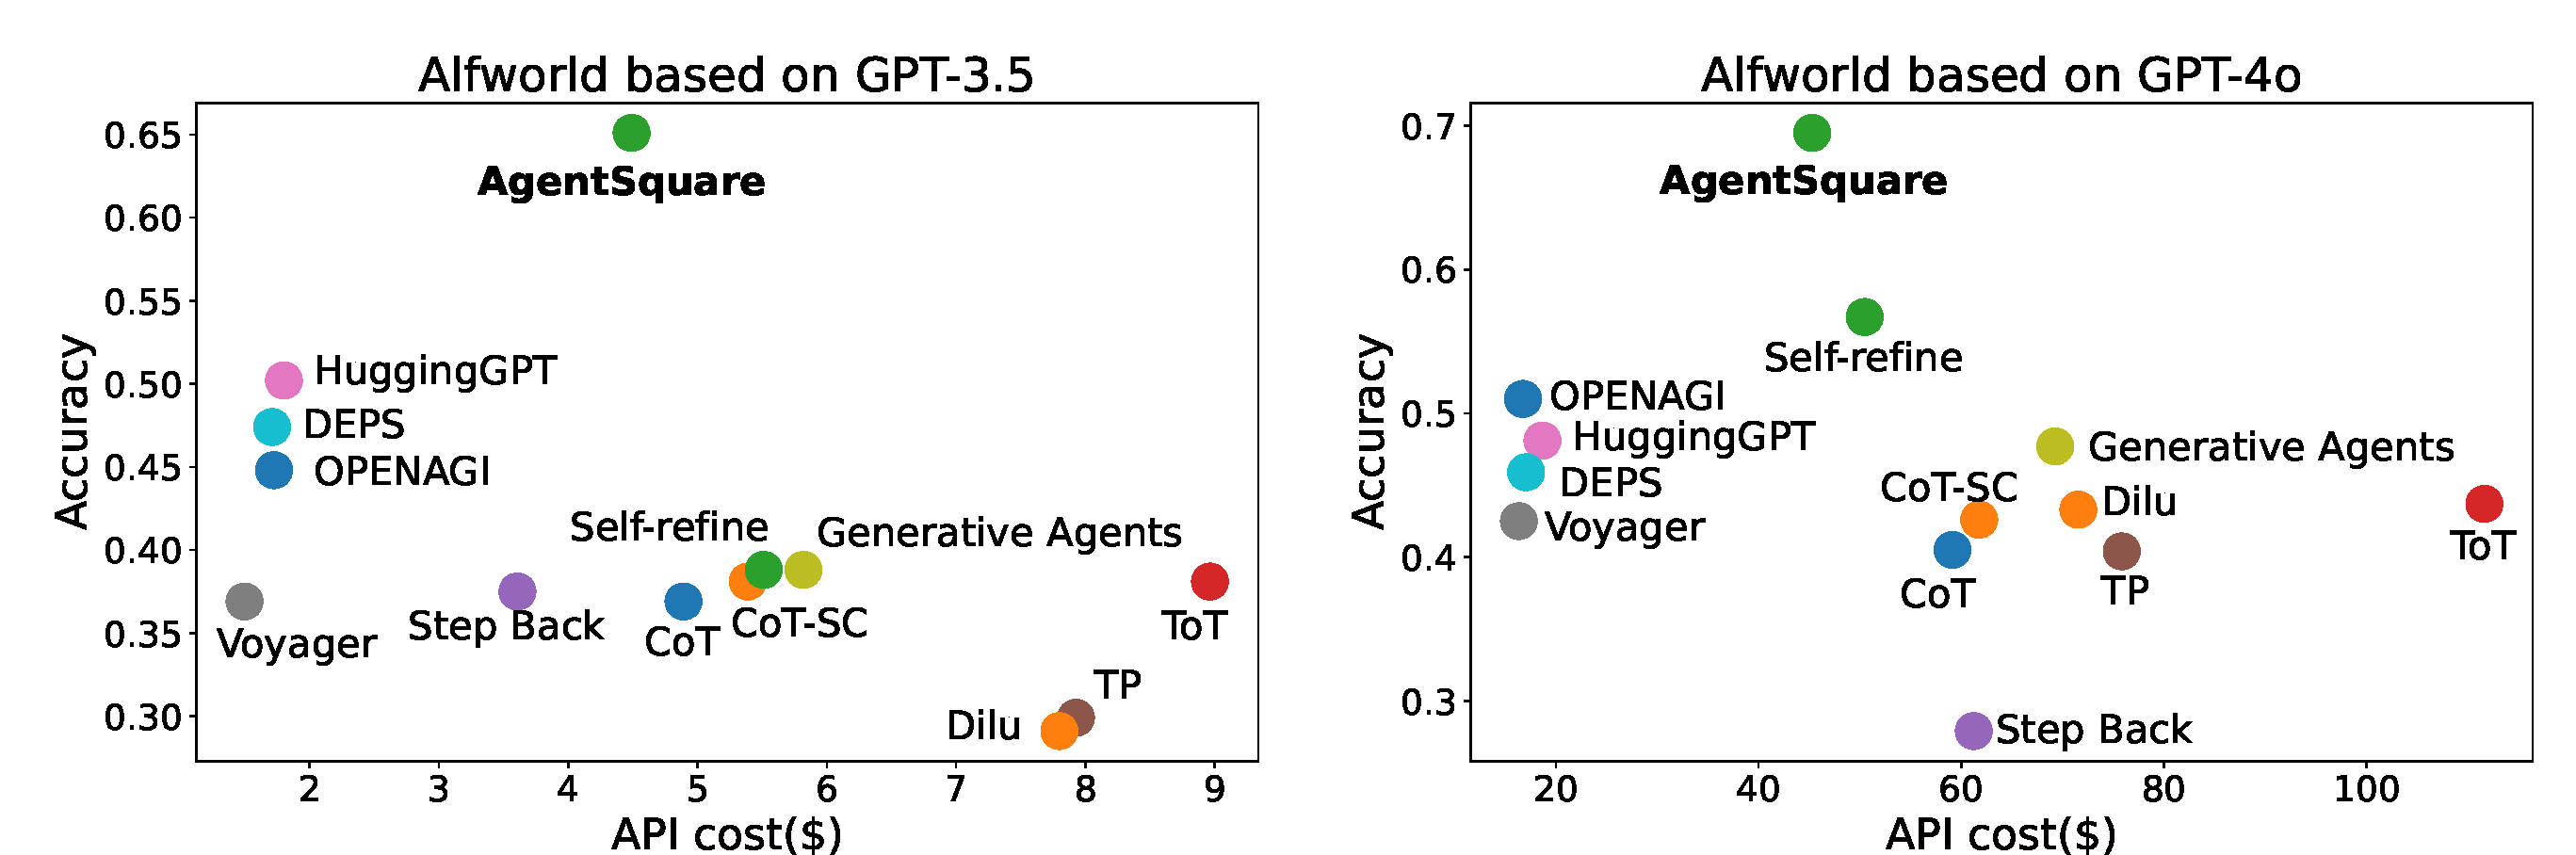
\includegraphics[width=\textwidth]{Figures/fig4_alfworld.pdf}
% % \includegraphics[width=12.5cm]{Figures/f4(sci).pdf}
% % \includegraphics[width=12.5cm]{Figures/f4(travel).pdf}
% %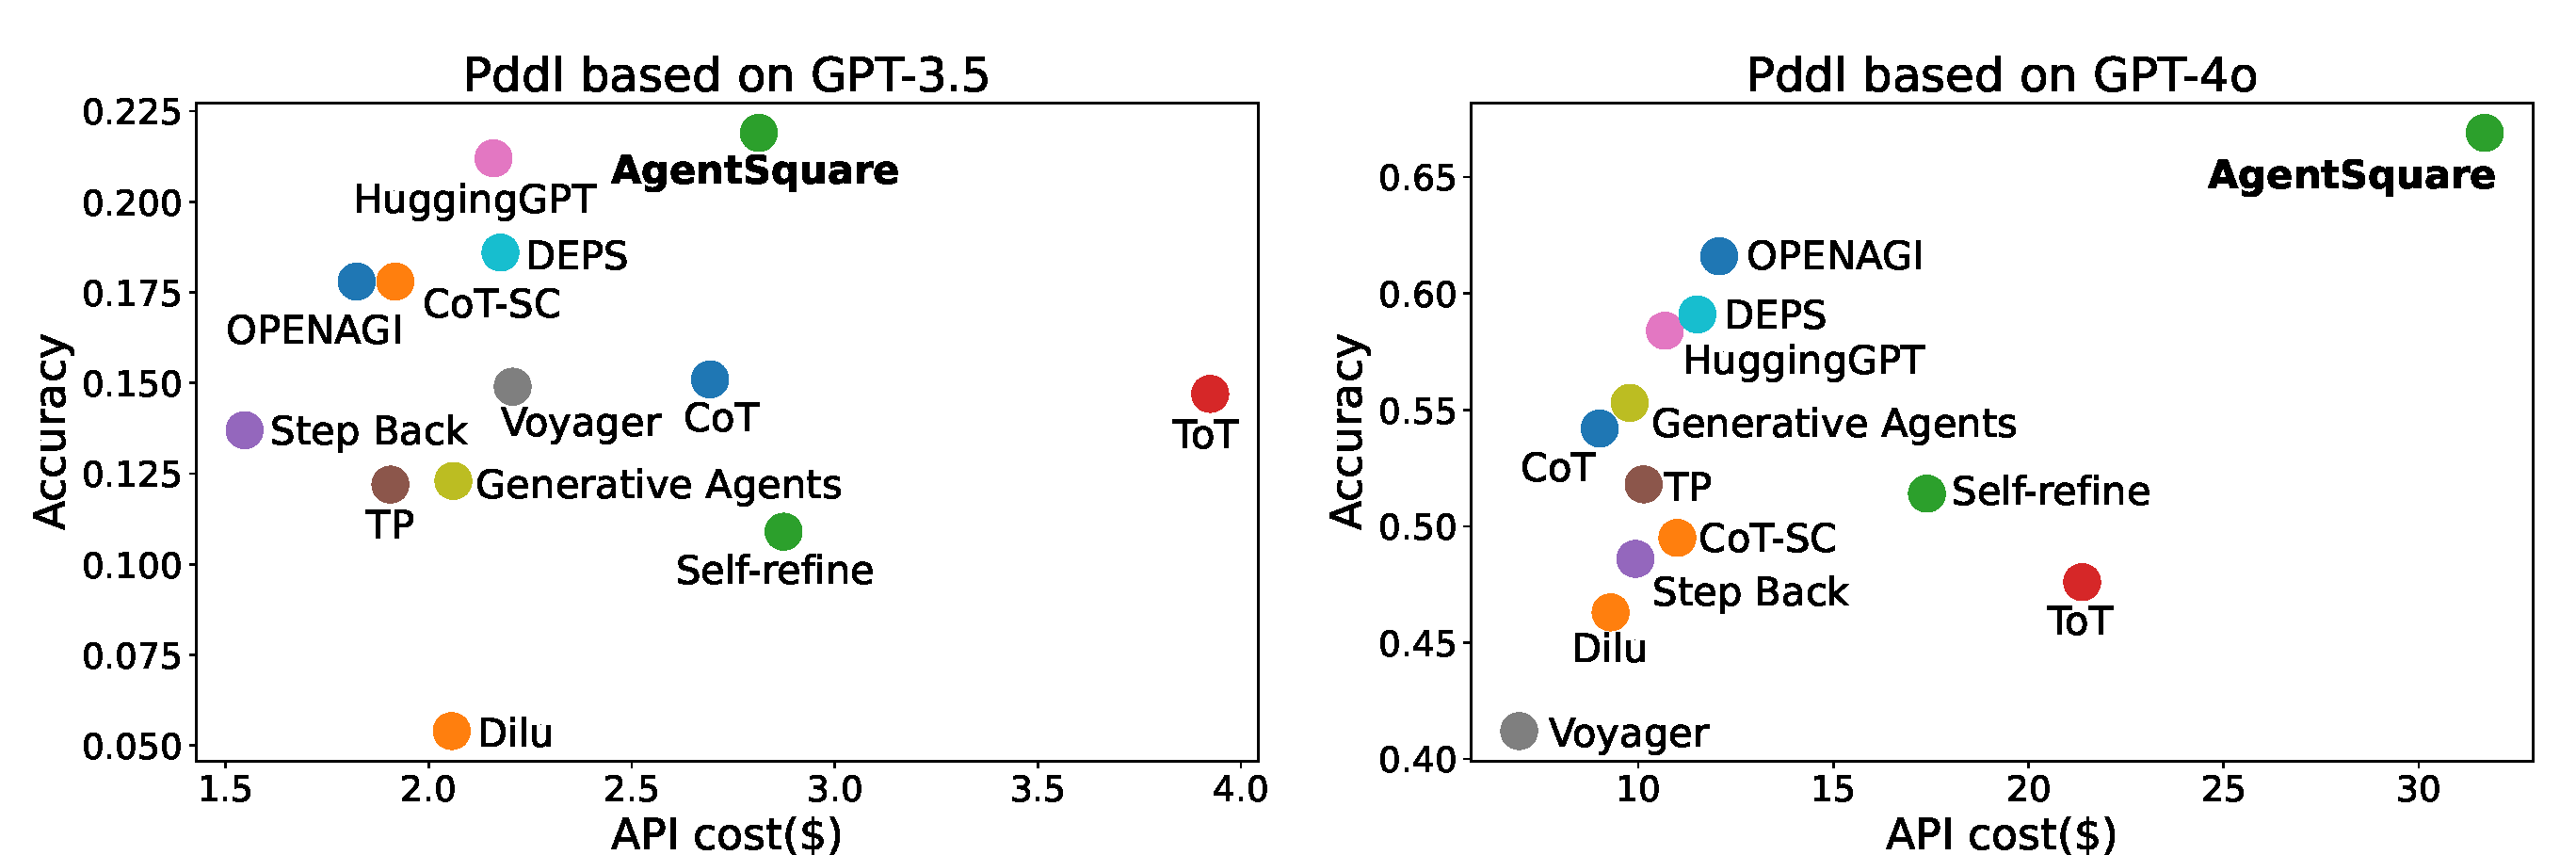
\includegraphics[width=12.5cm]{Figures/fig4_pddl.pdf}
% \caption{Performance versus API costs visualization on each task.}
% \label{fig4:performance-cost}
% \end{center}
% \end{figure}


\textbf{Search trajectory in AgentSquare.}
We present the search trajectory under 15 iterations using AgentSquare based on GPT-4o and other searching methods on ALFWorld and Webhop tasks in Figure~\ref{Fig7:trajectory}.
Results on other tasks are presented in Figure~\ref{app:trajectory1} and~\ref{app:trajectory2}.
AgentSquare demonstrates a steady convergence trajectory, where more advanced agents are continually emerging during search.
In contrast, module-level searching methods including random and Bayesian search lack a clear and insightful search direction.
Prompt-level search methods such as OPRO are constrained by a limited modification space, leading to minimal performance improvements.
As a result, they all encounter performance bottlenecks during the search process, resulting in sub-optimal agent architectures.
Besides, we find that simple module-level search methods such as random recombination greatly outperforms prompt-level search, indicating the importance of searching in the modular design space.  
\begin{figure}[!t]
\vspace{-6.5mm}
\begin{center}
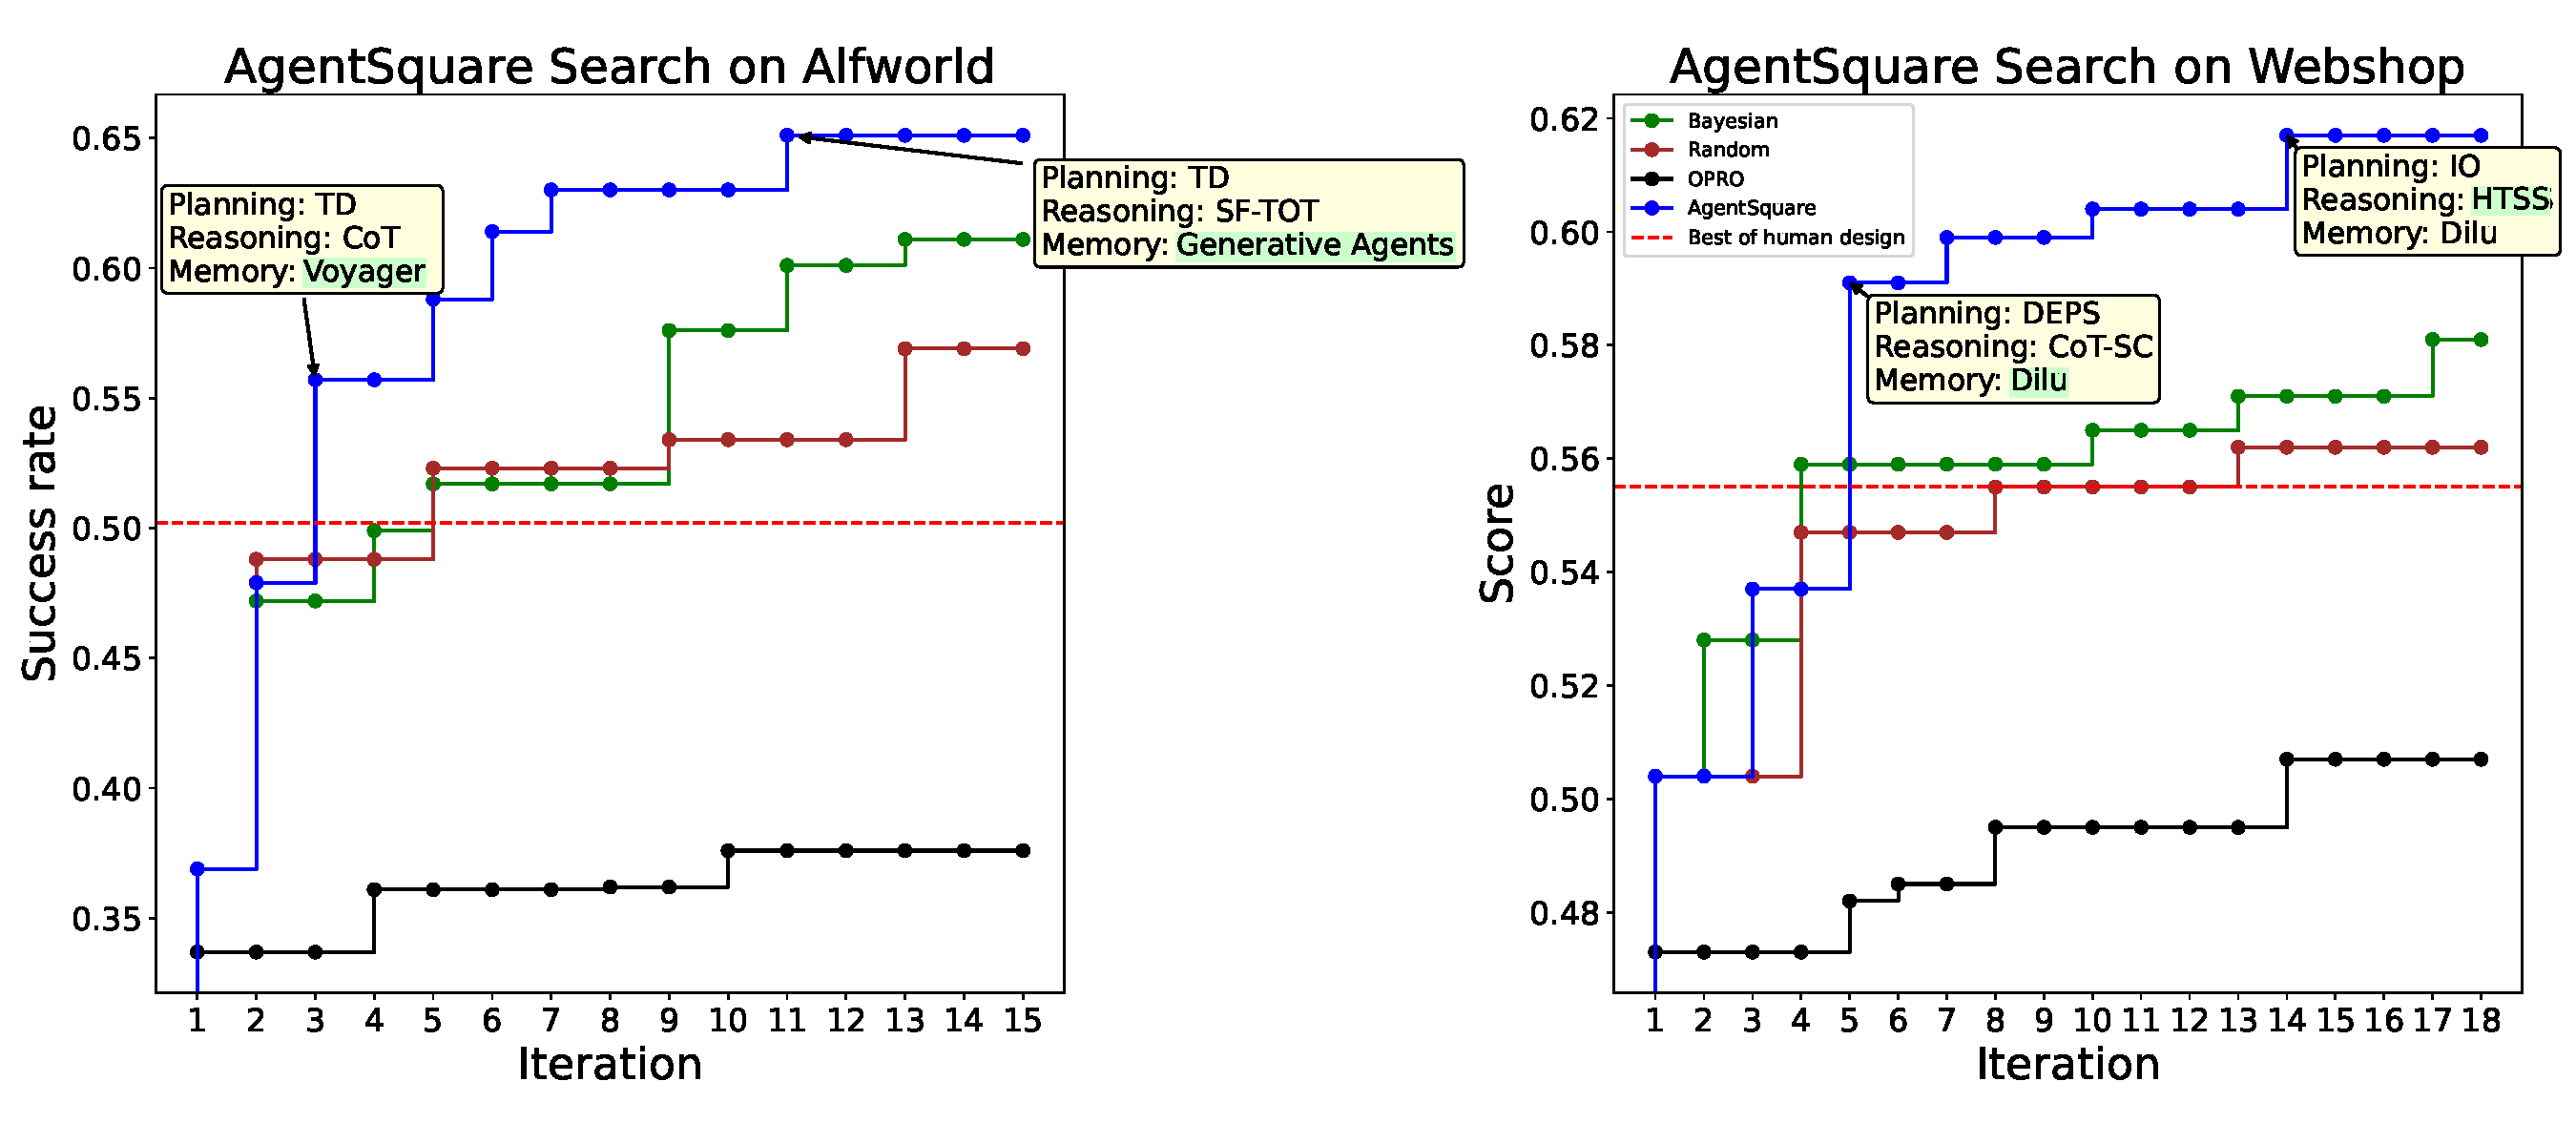
\includegraphics[width=0.8\textwidth]{Figures/fig5_alfworld_webshop.pdf}
\caption{AgentSquare search trajectory on Alfworld and Webshop.}
\vspace{-0.5em}
\label{Fig7:trajectory}
\end{center}
\end{figure}

\setlength{\tabcolsep}{1mm} 
\begin{table}[t!]
    \centering
    \begin{tabular}{cccccccc}
    \hline
    \textbf{Method} & \multicolumn{1}{c}{\textbf{Webshop}} & \multicolumn{1}{c}{\textbf{ALFWorld}} & \multicolumn{1}{c}{\textbf{SciWorld}} & \multicolumn{1}{c}{\textbf{M3Tool}} & \multicolumn{1}{c}{\textbf{TravelPlanner}}  
     & \multicolumn{1}{c}{\textbf{PDDL}}\\
    % \cmidrule(lr){2-5} \cmidrule(lr){6-9} \cmidrule(lr){10-12} \cmidrule(lr){13-15}
         % & Acc & Acc& Acc& Acc& Acc& Acc& Acc\\ 
    \hline
    AgentSquare (full) & \textbf{0.607} & \textbf{0.695} &\textbf{0.781}& \textbf{0.524} &\textbf{0.583}&\textbf{0.669}\\ 
    w/o module evolution& 0.564 & 0.649 &0.736& 0.502 &0.577 &0.614\\
    w/o module recombination& 0.560 & 0.616 &0.710& 0.481 &0.280 &0.669\\
    % w/o both-level search & 0.518 & 0.564 &0.704& 0.469 &0.563&0.558\\ 
    \hline
    \end{tabular}
    {\caption{Ablation study of AgentSquare on GPT-4o on six tasks across different domains.}
    \label{tab:ab2}}
\end{table}
\subsection{Ablation Study of AgentSquare} \label{technical}
\textbf{Effectiveness of module evolution and recombination.}
There are two key operations in the searching framework of AgentSquare: module evolution which creates new modules and module recombination which strategically recombines existing ones.
To verify the effectiveness of each design, we tested three variants: the full model, a version without module evolution, and a version without module recombination.
The results based on GPT-4o and GPT-3.5 are presented in Table~\ref{tab:ab2} and Table~\ref{tab:ab1}, respectively.
It can be seen that dropping each design results in a noticeable performance decline and the module recombination has a larger impact.
Module recombination significantly expands the search space, reducing the risk of falling into a local optima. 
Meanwhile, module evolution facilitates the discovery of more advanced modules tailored to specific tasks. 
These two operations collaborate well ensuring the effectiveness of the search process in AgentSquare.

\begin{figure}[!t]
\begin{center}
%\fbox{\rule[-.5cm]{0cm}{4cm} \rule[-.5cm]{4cm}{0cm}}
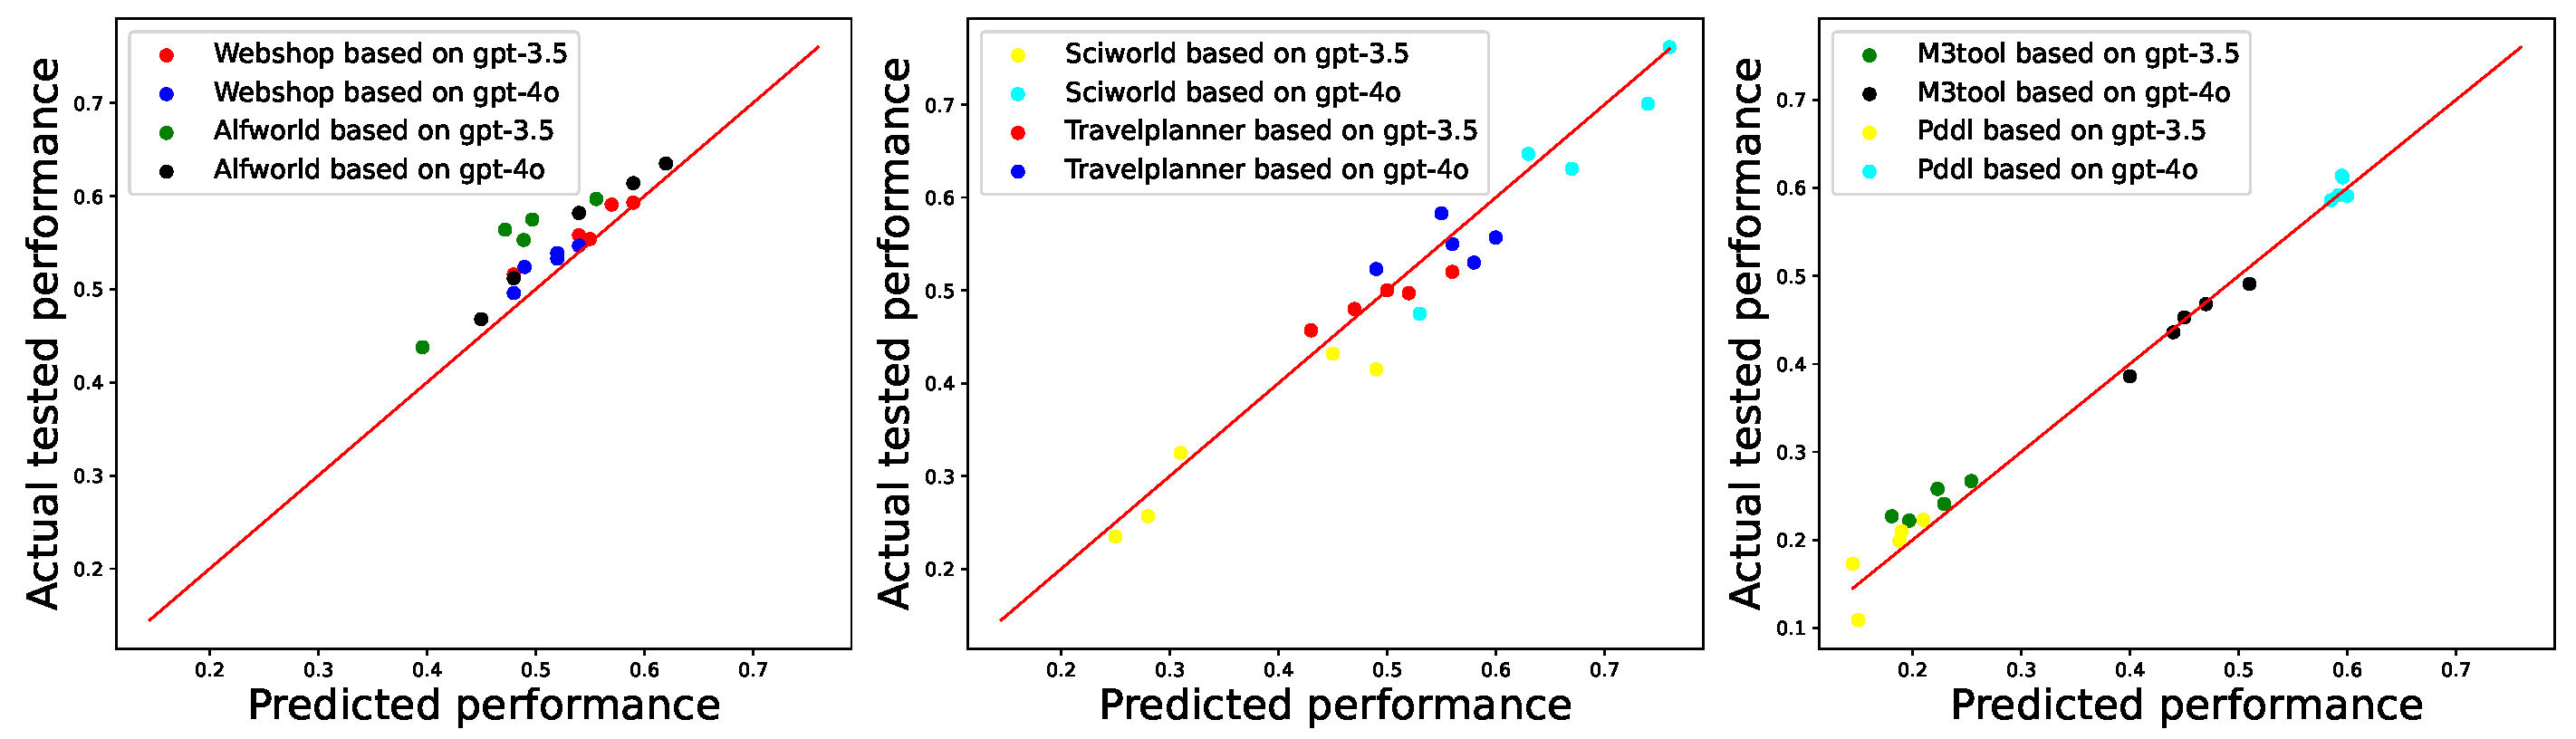
\includegraphics[width=0.85\textwidth]{Figures/fig6v0.pdf}
\caption{Validation of the effectiveness of the performance predictor (correlation between the actual and predicted performance) on each task.}
% \vspace{-3mm}
\label{pp}
\end{center}
\end{figure}

\textbf{Effectiveness of performance predictor.}
% To mitigate the high API costs associated with evaluating agents during the search process, we introduce an additional LLM as the performance predictor, inspired by existing practice utilizing LLM for neural architecture search~\citep{jawahar2023llm}.
In this part, we verify the effectiveness of this design empirically.
Figure~\ref{pp} illustrates the predicted performance of given agents versus their actual tested performance based on both GPT-3.5 and GPT-4o on all six tasks.
The tested agents were generated through random sampling by randomly combining existing modules. 
It can be found that the predicted performance closely aligns with the actual performance, demonstrating the effectiveness of the performance predictor.
For instance, the evaluation cost of the predictor is only about 0.025\% of the cost of a full evaluation based on GPT-4o in ALFWorld, demonstrating its remarkable cost-efficiency.
We provide more experiment results of predicting the performance of the dynamically searched agents in Figure~\ref{pp-search} of the Appendix.
\subsection{Discovered Best Agents from AgentSquare}
In this section, we provide some illustrations of the searched best agents, especially some discovered promising modules.
Table~\ref{tab:module} summarizes the searched best agent from AgentSquare and the best hand-crafted agents on all tasks.
We can observe that AgentSquare can adaptively identify promising agents with both previously existing and newly programmed modules tailored to the given task.
For instance, the discovered best agent for ALFWorld combines an existing well-designed memory module from \textit{Generative Agents} with newly created planning (named \textit{TD}) and reasoning modules (named \textit{SF-ToT}). 
By comparison, the best hand-crafted agent \textit{Self-refine} focuses only on reasoning module design while overlooking other functional modules, leading to suboptimal performance.
Moreover, we illustrate two new modules and the human interpretable design insights discovered on ALFWorld in Figure~\ref{main:New module}.
More illustrations are listed in the Figure~\ref{New module1} to Figure~\ref{New module6}.


% \setlength{\tabcolsep}{1.mm}         
% \begin{table}[t!]
%     \centering
%     \begin{tabular}{ccccc|c}
%     \hline
%     \textbf{Task} & \textbf{Planning} & \textbf{Reasoning} & \textbf{Tooluse} & \textbf{Memory} & \textbf{Best Hand-crafted Agents} \\ \hline
%     Webshop & IO & HTSS & / & Dilu & HuggingGPT \\ \hline
%     ALFWorld & TD & SF-ToT & / & Generative Agents& Self-refine \\ \hline
%     SciWorld & Voyager& CoT& / & Hier& Voyager\\ \hline
%     M3Tool & / & CoT-SC & ToolBF & / & Toolbench \\ \hline
%     TravelPlanner & DEPS & CoT & TH & / & DEPS \\ \hline
%     PDDL & IR & CASRC & / & Generative Agents& OPENAGI \\ \hline
%     \end{tabular}
%     {\caption{Comparison between the searched best agent from AgentSquare and the best human-designed agent on all tasks.}
%     \label{tab:module}}
% \end{table}

\begin{figure}[!t]
\begin{center}
%\fbox{\rule[-.5cm]{0cm}{4cm} \rule[-.5cm]{4cm}{0cm}}
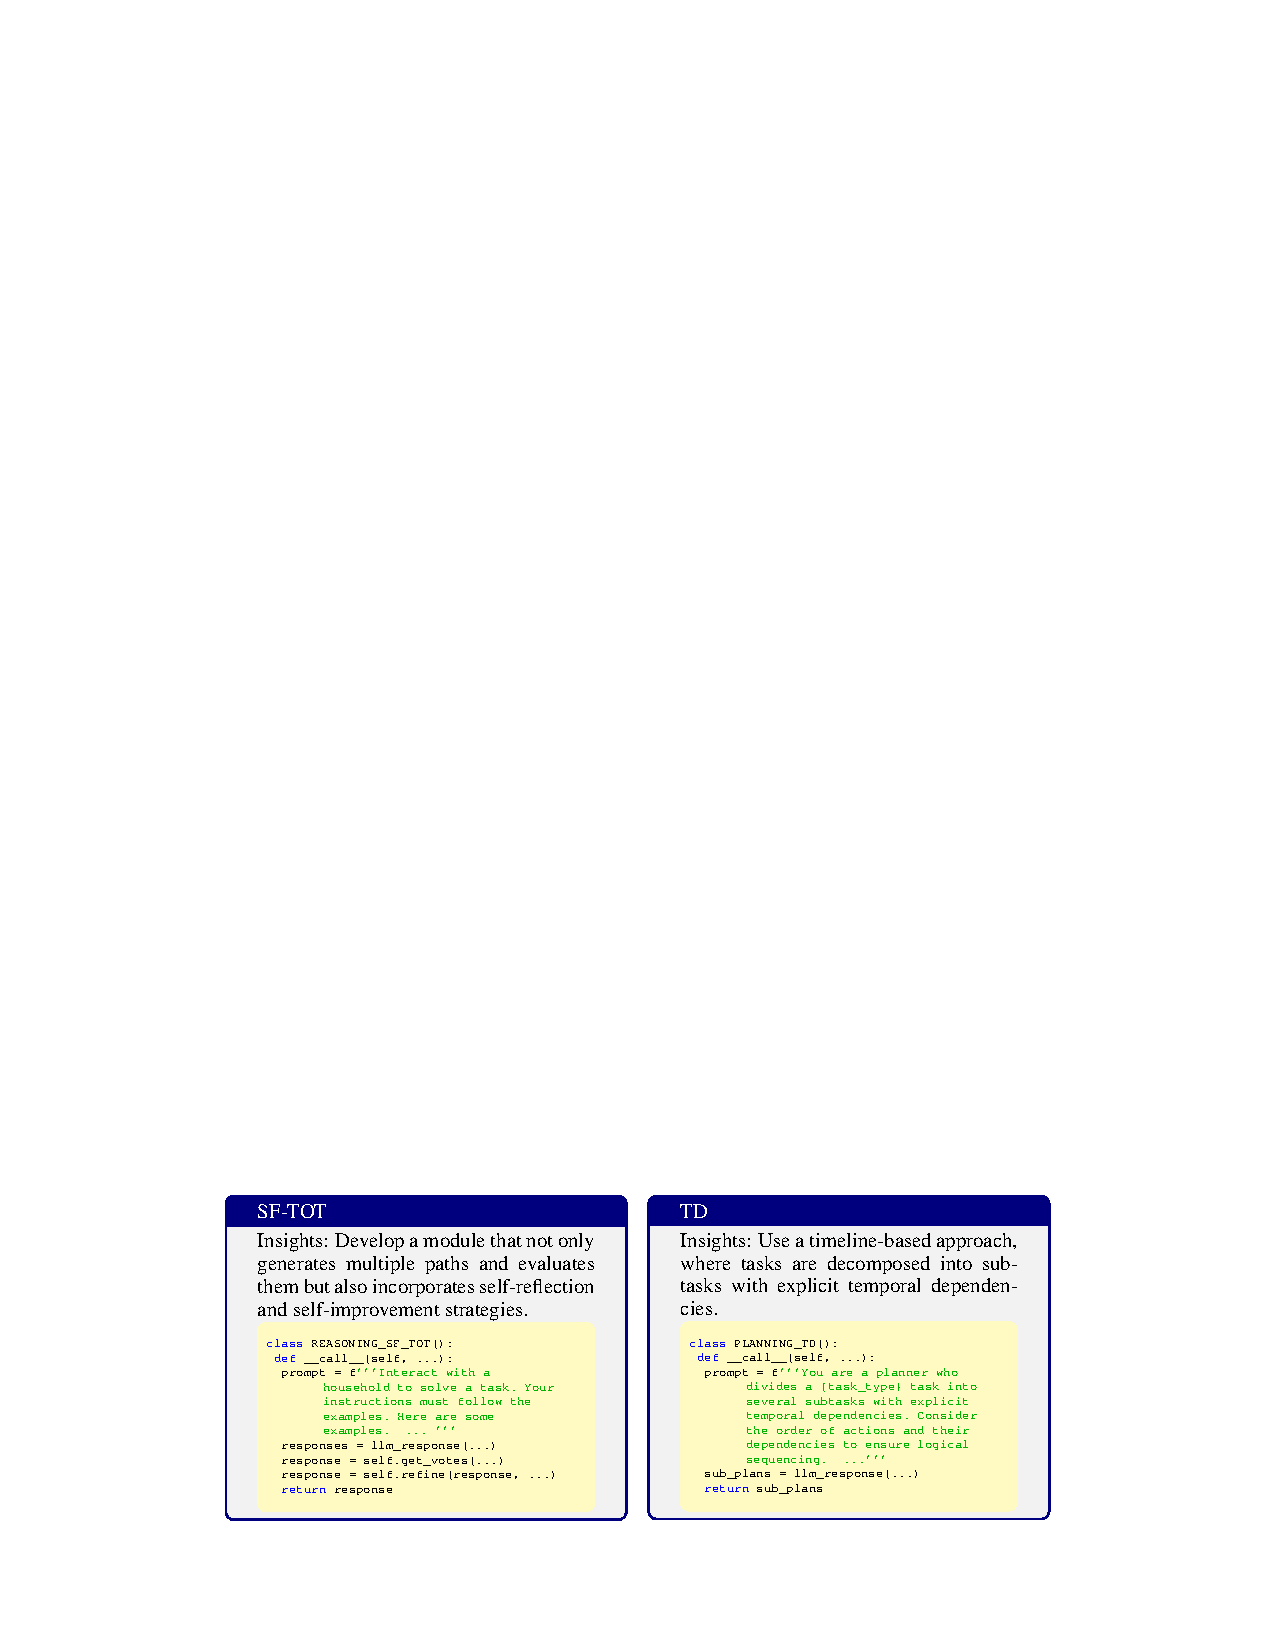
\includegraphics[width=0.8\textwidth]{Figures/new_module_alfworld.pdf}
\caption{New module discovered through AgentSquare search on ALFWorld.}
\label{main:New module}
\end{center}
\end{figure}



% \setlength{\tabcolsep}{1.5mm} 
% \begin{table}[t!]
%     \centering
%     \begin{tabular}{cccccccc}
%     \hline
%     \textbf{Method} & \multicolumn{1}{c}{\textbf{Webshop}} & \multicolumn{1}{c}{\textbf{ALFWorld}} & \multicolumn{1}{c}{\textbf{SciWorld}} & \multicolumn{1}{c}{\textbf{M3Tool}} & \multicolumn{1}{c}{\textbf{TravelPlanner}} & 
%      \multicolumn{1}{c}{\textbf{PDDL}}\\
%     % \cmidrule(lr){2-5} \cmidrule(lr){6-9} \cmidrule(lr){10-12} \cmidrule(lr){13-15}
%          % & Acc & Acc& Acc& Acc& Acc& Acc& Acc\\ 
%     \hline
%         % IO & 0.473 & 0.306 & 0.105& 0.158  &0.043 & 0.166\\ 
%         CoT & 0.504 & 0.369 & 0.142 & 0.172 &0.080& 0.151\\ 
%         CoT-SC & 0.527 & 0.381 & 0.105& 0.181  & 0.167& 0.178\\ 
%         Self-refine & 0.439 & 0.388 & 0.222& 0.098  & 0.000& 0.109\\ 
%         ToT & 0.510 & 0.381 & 0.143 & 0.189  & 0.163& 0.147\\ 
%         Step Back & 0.478 & 0.375 &0.027& 0.128  & 0.120& 0.137\\ 
%         Thought Propagation & 0.429 & 0.299 &0.168& 0.139  & 0.063 & 0.122\\ 
%         % toolformer & / & / & /& 0.194  & 0.000& / \\ 
%         % toolbench & / & / & /& 0.204  & 0.053& / \\ 
%         % anytool & / & / & /& 0.139  & 0.077&  / \\ 
%         HuggingGPT & 0.518 & 0.502 & 0.27& 0.012  &0.470 & 0.212 \\ 
%         Voyager & 0.427 & 0.369 & 0.301& 0.008&0.480 &0.149\\ 
%         Generative Agents & 0.539 & 0.388 & 0.153& 0.144  & 0.060& 0.123 \\ 
%         DEPS & 0.555 & 0.474 & 0.308 & 0.017  & 0.500& 0.186\\ 
%         OPENAGI & 0.507 & 0.448 & 0.257 & 0.008  & 0.430& 0.178\\ 
%         Dilu & 0.418 & 0.291 &0 & 0.131 &0.137 &0.054\\ 
%         Random Recombination & & & & & & \\
%         Bayesian Recombination & & & & & & \\
%         PromptBreeder & & & & & &  \\
%         OPRO & & & & & & \\
%    \textbf{AgentSquare} & 0.617 & 0.651 &0.432& 0.285&0.520&0.219 \\ \hline
%     \end{tabular}
%     {\caption{Performance comparison of searched agents from AgentSquare and existing human-designed agents based on GPT-3.5 on six tasks across different domains (add task domains).}
%     \label{tab:main1}}
% \end{table}




% \setlength{\tabcolsep}{1.5mm} 
% \begin{table}[t!]
%     \centering
%     \begin{tabular}{cccccccc}
%     \hline
%     \textbf{Method} & \multicolumn{1}{c}{\textbf{Webshop}} & \multicolumn{1}{c}{\textbf{ALFWorld}} & \multicolumn{1}{c}{\textbf{SciWorld}} & \multicolumn{1}{c}{\textbf{M3Tool}} & \multicolumn{1}{c}{\textbf{TravelPlanner}} & 
%      \multicolumn{1}{c}{\textbf{PDDL}}\\
%     % \cmidrule(lr){2-5} \cmidrule(lr){6-9} \cmidrule(lr){10-12} \cmidrule(lr){13-15}
%          % & Acc & Acc& Acc& Acc& Acc& Acc& Acc\\ 
%     \hline
%         % IO & 0.411 & 0.367 & 0.759& 0.439 & 0.407& 0.559\\ 
%         CoT & 0.485 & 0.405 & 0.697& 0.448  & 0.487 & 0.542\\ 
%         Cot-SC & 0.512 & 0.426 & 0.656 & 0.461  & 0.413& 0.495\\ 
%         Self-refine & 0.461 & 0.567 & 0.654 & 0.442  & 0.000& 0.514\\ 
%         ToT & 0.501 & 0.437 & 0.741& 0.453  &0.380 & 0.476\\ 
%         Step Back & 0.468 & 0.279 & 0.220 & 0.434  & 0.000& 0.486\\ 
%         Thought Propagation & 0.398 & 0.404 & 0.576 & 0.387  & 0.430& 0.518\\ 
%         % toolformer & / & / & / & 0.449  & 0.510& / \\ 
%         % toolbench & / & / & /& 0.469  & 0.000 &  / \\ 
%         % anytool & / & / & / & 0.375  & 0.523& / \\ 
%         HuggingGPT & 0.519 & 0.481 & 0.680& 0.354  & 0.510& 0.584\\ 
%         Voyager & 0.366 & 0.425 & 0.776& 0.247 &0.523 &0.412\\ 
%         Generative Agents & 0.499 & 0.477 & 0.663& 0.402  & 0.480& 0.553\\ 
%         DEPS & 0.481 & 0.459 & 0.740 & 0.278 & 0.540& 0.591\\ 
%         OPENAGI & 0.506 & 0.510 & 0.718& 0.322  & 0.533 & 0.616\\ 
%         Dilu & 0.451 & 0.433 & 0.682 & 0.475 &0.360 &0.463\\ 
%         Random Recombination & & & & & & \\
%         Bayesian Recombination & & & & & & \\
%         PromptBreeder & & & & & &  \\
%         OPRO & & & & & & \\
%     \textbf{AgentSquare} & 0.607 & 0.695 & 0.781& 0.524 &0.583 &0.669\\  \hline
%     \end{tabular}
%     {\caption{Performance comparison of searched agents from AgentSquare and existing human-designed agents based on GPT-4 on six tasks across different domains.}
%     \label{tab:main2}}
% \end{table}






% \begin{figure}[!t]
% \begin{center}
% \fbox{\rule[-.5cm]{0cm}{4cm} \rule[-.5cm]{4cm}{0cm}}
% \caption{Analysis for LLM agent design choices in 4 dimensions over different tasks.}
% \label{module-level}
% \end{center}
% \end{figure}

% \setlength{\tabcolsep}{3mm}         
% \begin{table}[t!]
%     \centering
%     \begin{tabular}{cccccc}
%     \hline
%     \textbf{Task} & \textbf{Agent Type} &\textbf{Planning} & \textbf{Reasoning} & \textbf{Tooluse} & \textbf{Memory} \\ \hline
%     \multirow{2}{*}{Webshop} & Hand-crafted Agents & hugginggpt & IO & / & / \\
%                              & AgentSquare search & IO & cot-sc & / & dilu \\ \hline
%     \multirow{2}{*}{ALFWorld} & Hand-crafted Agents & / & self-refine & / & / \\
%                              & AgentSquare search & RP & SF_TOT & / & generative \\ \hline
%     \multirow{2}{*}{SciWorld} & Hand-crafted Agents &DEPS &IO &/&/ \\
%                              & AgentSquare search &Adaptive &IO &/&/ \\ \hline
%     \multirow{2}{*}{M3Tool} & Hand-crafted Agents & / & / & toolbench & / \\
%                              & AgentSquare search & / & cot-sc & toolbench & / \\ \hline
%     \multirow{2}{*}{TravelPlanner} & Hand-crafted Agents &DEPS &IO &IO&/ \\
%                                    & AgentSquare search &DEPS &COT &TH&/ \\ \hline
%     \multirow{2}{*}{PDDL} & Hand-crafted Agents &OPENAGI & IO &/ & / \\
%                           & AgentSquare search &self-refine-COT & Iterative-refine&/&generative \\ \hline
%     \end{tabular}
%     {\caption{Comparison between the searched best agent from AgentSquare and the best human-designed agent on all tasks (show prompts of searched modules, only show the best human-design agent's name).}
%     \label{tab:main2}}
% \end{table}

% \setlength{\tabcolsep}{1.mm}         
% \begin{table}[t!]
%     \centering
%     \begin{tabular}{ccccc|c}
%     \hline
%     \textbf{Task} & \textbf{Planning} & \textbf{Reasoning} & \textbf{Tooluse} & \textbf{Memory} & \textbf{Best Hand-crafted Agents} \\ \hline
%     Webshop & IO & HTSS & / & Dilu & HuggingGPT \\ \hline
%     ALFWorld & RP & SF-TOT & / & Generative Agents& Self-refine \\ \hline
%     SciWorld & Adaptive & IO & / & / & DEPS \\ \hline
%     M3Tool & / & CoT-SC & ToolBF & / & Toolbench \\ \hline
%     TravelPlanner & DEPS & COT & TH & / & DEPS \\ \hline
%     PDDL & Self-refine-COT & Iterative-refine & / & Generative Agents& OPENAGI \\ \hline
%     \end{tabular}
%     {\caption{Comparison between the searched best agent from AgentSquare and the best human-designed agent on all tasks (show prompts of searched modules).}
%     \label{tab:main2}}
% \end{table}


% \setlength{\tabcolsep}{1mm} 
% \begin{table}[t!]
%     \centering
%     \begin{tabular}{cccccccc}
%     \hline
%     \textbf{Method} & \multicolumn{1}{c}{\textbf{Webshop}} & \multicolumn{1}{c}{\textbf{ALFWorld}} & \multicolumn{1}{c}{\textbf{SciWorld}} & \multicolumn{1}{c}{\textbf{M3Tool}} & \multicolumn{1}{c}{\textbf{TravelPlanner}}  
%      & \multicolumn{1}{c}{\textbf{PDDL}}\\
%     % \cmidrule(lr){2-5} \cmidrule(lr){6-9} \cmidrule(lr){10-12} \cmidrule(lr){13-15}
%          % & Acc & Acc& Acc& Acc& Acc& Acc& Acc\\ 
%     \hline
%     AgentSquare (full) & \textbf{0.617} & \textbf{0.651} &\textbf{0.432}& \textbf{0.285} &\textbf{0.520}&\textbf{0.219}\\ 
%     w/o module evolution& 0.595 & 0.623 &0.288& 0.236 &0.483&0.202 \\
%     w/o module recombination& 0.578 & 0.546 &0.310& 0.258 & 0.267&0.173\\
%     % w/o both-level search& 0.555 & 0.512 &0.367& 0.204 &0.473&0.159 \\ 
%     \hline
%     \end{tabular}
%     {\caption{Ablation study of AgentSquare on GPT-3.5 on six tasks across different domains.}
%     \label{tab:ab1}}
% \end{table}

